$subject$=Физические основы компьютерных \\ и сетевых технологий
$teacher$=Решение задач из сборника
$date$=

\clearpage

\section{Y. Решение задач из сборника}

\subsection{Электромагнетизм}

\begin{tcolorbox}
    \textbf{Задача 1.4.2.} Три одинаковых одноименных заряда $q$
    расположены в вершинах равностороннего треугольника. Какой
    заряд $Q$ противоположного знака нужно поместить в центр этого
    треугольника, чтобы результирующая сила, действующая на
    каждый заряд, была равна нулю?
\end{tcolorbox}

\begin{minipage}{\textwidth}
    \begin{wrapfigure}{r}{0pt}
        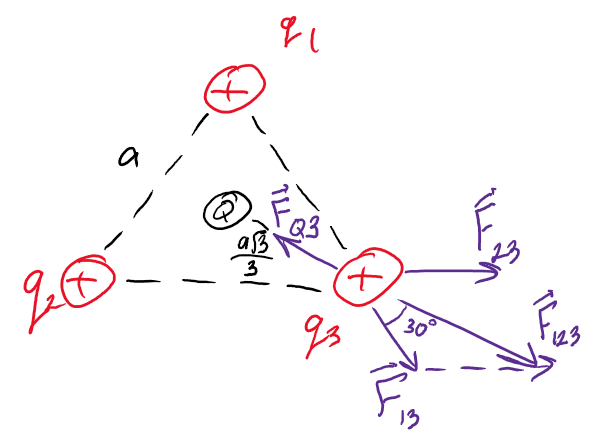
\includegraphics[width=8cm]{physics1/images/physics1_homework_6_1}
    \end{wrapfigure}

    Чтобы результирующая сила, действующая на каждый заряд, была равна нулю, сумма сил, 
    действующих на каждый заряд от других зарядов, должна быть равна нулю.

    Так как на заряд $Q$ в центре действуют одинаковая сила со всех других зарядов, то в силу симметрии его суммарная сила равна 0 

    Возьмем заряд $q_3$ в вершине - на него действуют три силы: $\vec{F}_{13}, \vec{F}_{23}$ и $\vec{F}_{Q3}$

    $F_{13} = F_{23} = \frac{kq}{a^2}$

    Результирующая сил сила $F_{123} = 2F_{13} \cdot \cos 30^\circ = \sqrt{3}\frac{kq}{a^2}$

    $F_{Q3} = \frac{kQ}{\left(\frac{a\sqrt{3}}{3}\right)^2} = \frac{3kQ}{a^2}$

    $F_{Q3} = F_{123} \Longrightarrow \sqrt{3}\frac{kq}{a^2} = \frac{3kQ}{a^2} \Longrightarrow Q = \frac{\sqrt{3}q}{3}$
\end{minipage}

\underline{Ответ}: $\frac{\sqrt{3}q}{3}$


\clearpage

\begin{tcolorbox}
    \textbf{Задача 1.4.9.} Точечный заряд $q$ находится в центре тонкого
    кольца радиуса $R$, по которому равномерно распределен заряд $(—q)$.
    Найти модуль вектора напряженности электрического поля на оси
    кольца в точке, отстоящей от центра кольца на расстояние $x \gg R$.
\end{tcolorbox}

\begin{minipage}{\textwidth}
    \begin{wrapfigure}{r}{0pt}
        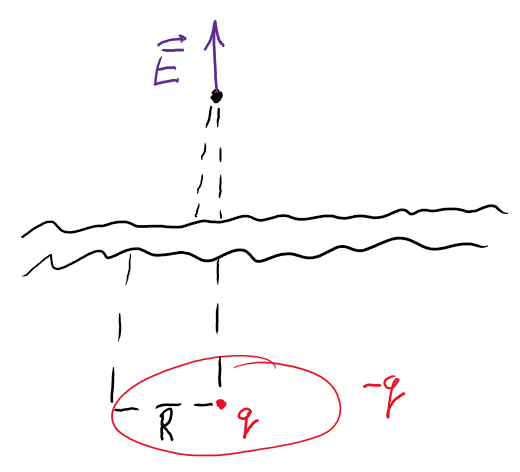
\includegraphics[width=8cm]{physics1/images/physics1_homework_6_2}
    \end{wrapfigure}

    На лекции выводили формулу напряженности кольца в точке, расположенной на оси кольца: 

    $E_{\text{кольца}} = -\frac{kqx}{(R^2 + x^2)^{\frac{3}{2}}}$

    При $x \gg R$ можем сказать, что $(R^2 + x^2) \approx x^2$ - тогда получаем, что кольцо можно представить как точечный заряд:

    $E_{\text{кольца}} \approx -\frac{kq}{x^2}$

    Аналогично для точечного заряда получаем 
    
    $E_{\text{т.з.}} = \frac{kq}{x^2}$
\end{minipage}

Получаем напряженность в точке $E = E_{\text{т.з.}} + E_{\text{кольца}} = 0$
\footnote{Несмотря на это, можно получить более точную оценку: \\
$E = \frac{kq}{x^2} \left(1 - \frac{1}{\left(\frac{R^2}{x^2} + 1\right)^{\frac{3}{2}}}\right) \approx \left[\text{делаем замену } y = \frac{R^2}{x^2}, \text{ разложение } \left(1 - \frac{1}{(y + 1)^{\frac{3}{2}}}\right) \text{ по Тейлору}\right] \approx \frac{3kqR^2}{2x^4}$}

\underline{Ответ}: 0

\clearpage

\begin{tcolorbox}
    \textbf{Задача 1.4.11.} Система состоит из тонкого заряженного
    проводящего кольца радиуса $R$ и очень длинной нити, равномерно
    заряженной с линейной плотностью $\tau$, расположенной на оси
    кольца так, что один из её концов совпадает с центром кольца.
    Кольцо имеет заряд $q$. Найти силу взаимодействия кольца и нити.
\end{tcolorbox}

\begin{minipage}{\textwidth}
    \begin{wrapfigure}{r}{0pt}
        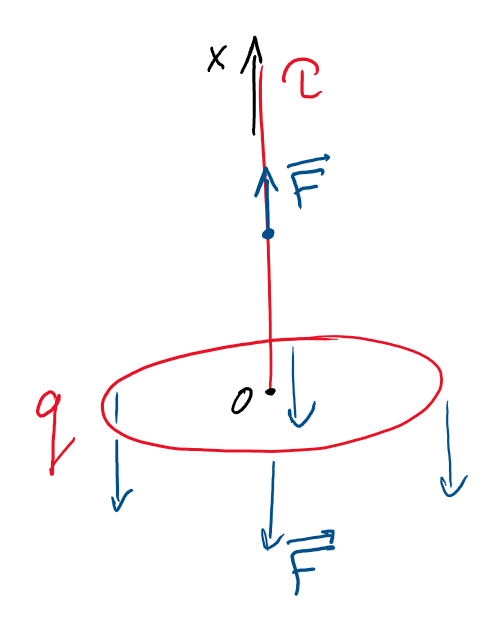
\includegraphics[width=8cm]{physics1/images/physics1_homework_6_3}
    \end{wrapfigure}

    Формула напряженности кольца в точке, расположенной на оси кольца: 

    $E_{\text{кольца}} = \frac{kqx}{(R^2 + x^2)^{\frac{3}{2}}}$

    Тогда для каждого кусочка заряда $d\tilde{q}$ на нити сила равна

    $dF = d\tilde{q} E_{\text{кольца}} = d\tilde{q} \frac{kqx}{(R^2 + x^2)^{\frac{3}{2}}}$

    Для всей нити получаем: 

    $F = \int_l d\tilde{q} \frac{kqx}{(R^2 + x^2)^{\frac{3}{2}}} = \int_0^\infty \frac{kqx}{(R^2 + x^2)^{\frac{3}{2}}} \tau dx = 
    \frac{k\tau q}{2} \frac{-2}{\sqrt{R^2 + x^2}} \Big|_0^\infty = \frac{k\tau q}{R}$
\end{minipage}

\underline{Ответ}: $\frac{k\tau q}{R}$

\clearpage

\begin{tcolorbox}
    \textbf{Задача 1.4.14.} Шар радиуса $R$ сферически симметрично
    заряжен по объему зарядом $Q$ так, что $p(r) \sim r^2$. Определить
    напряженность электрического поля в точках $A$ и $B$, если $r_A = 0.5R$,
    a $r_B=2R$.
\end{tcolorbox}


\begin{minipage}{\textwidth}
    \begin{wrapfigure}{r}{0pt}
        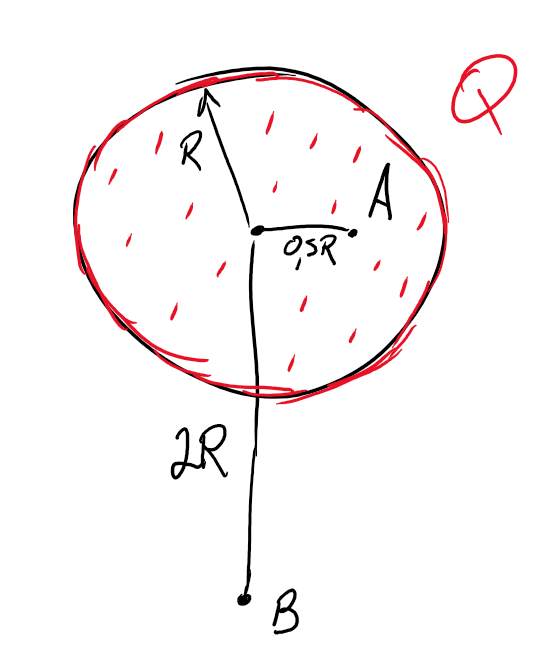
\includegraphics[width=8cm]{physics1/images/physics1_homework_6_4}
    \end{wrapfigure}

    Пусть $\rho(r) = mr^2$, где $m$ некая константа, тогда 

    $Q = \iiint \rho(r) dV = \int_0^R \rho(r) S(r) dr = \int_0^R mr^2 \cdot 4\pi r^2 \cdot dr = \frac{4}{5}m\pi R^5$

    Из этого $m = \frac{5Q}{4\pi R^5}, \rho(r) = r^2\frac{5Q}{4\pi R^5}$

    Для точки $B$ воспользуемся выкладками из лекции, в точке вне шара напряженность можем считать по формуле
    точечного заряда:

    $E_B = k\frac{Q}{4R^2}$

    Теперь найдем $q(r)$ - количество заряда внутри сферы радиуса $r$:

    $q(r) = \int_0^r \rho(t) S(t) dt = \int_0^r mt^2 \cdot 4\pi t^2 \cdot dr = \frac{4}{5}m\pi r^5 = Q\frac{r^5}{R^5}$

    По теореме Гаусса $E_A S(r) = \frac{q(r)}{\varepsilon_0}$, тогда 

    $E_A = Q\frac{r^5}{R^5} \frac{1}{4\pi\varepsilon_0 r^2} = kQ\frac{r^3}{R^5} = \frac{kQ}{8R^2}$

\end{minipage}

\underline{Ответ}: $E_A = \frac{kQ}{8R^2}, E_B = k\frac{Q}{4R^2}$


\clearpage
